\chapter{Q01}
\emph{Q1: Explain the architecture and primary tasks of a WSN node? What are
the main HW sub-components characteristics? Give an example of one or two
existing WSN node families.}

\section{Arkitektur og opgaver for en mote}

\begin{description}
\item Sensing.
\item Processing.
\item Communication.
\end{description}

\section{HW del-komponenter}

\begin{figure}[h]
  \centering
  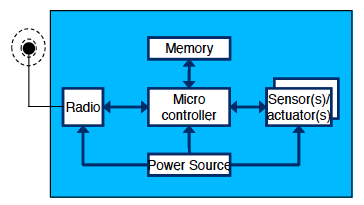
\includegraphics[scale=0.5]{img/moteAnatomy.png}
  \caption{Architecture.}
\end{figure}

\subsection{Sensors}
\begin{description}
\item[Passive omnidirectional] Fx: light, thermometer, microphones.
\item[Passive narrowbeam] Fx: camera.
\item[Active] Radar
\end{description}

\begin{description}
\item Digital interface.
\item Analog interface voltage.
\end{description}

\subsection{Controller}

\begin{description}
\item Execute programs
\item Process tasks.
\end{description}

Goals.

\begin{description}
\item Flexibility.
\item Performance.
\item Energy efficient.
\item Cost.
\end{description}

\subsection{Communication}
\begin{description}
\item Light, electromagnetic.
\item Ultrasound.
\item Radio Frequency (RF).
\end{description}

States.
\begin{description}
\item Transmit.
\item Receive.
\item Idle.
\item Sleep.
\end{description}

\subsection{Memory}

\begin{description}
\item Store programs, data.
\item Variable data in SRAM -> Volatile.
\item On-chip memories.
\item External flash.
\end{description}

\subsection{Energy}
\begin{description}
\item Storage.
\item Distribution / management.
\item Harvesting.
\end{description}
\section{Eksempler på node familier}



%%% Local Variables: 
%%% mode: latex
%%% TeX-master: "../master"
%%% End: 
